\documentclass[11pt,a4paper]{article}
\usepackage[margin=1.8cm]{geometry}
\usepackage{amsmath,amssymb,booktabs,graphicx,array,longtable}
\usepackage[hidelinks]{hyperref}
\usepackage{microtype}
\setlength{\parindent}{0pt}
\setlength{\parskip}{0.45em}
\graphicspath{{figures/}}
\newcommand{\pt}{p_{\mathrm T}}
\newcommand{\mc}{\mathrm{MC}}
\newcommand{\ttW}{t\bar tW^+}
\newcommand{\code}[1]{\texttt{\detokenize{#1}}}
\title{Production--decay scale correlations and width conventions\\
in on-shell trileptonic $t\bar tW^+$ production}
\author{ttW production--decay study}
\date{19 October 2026}
\begin{document}
\maketitle
\begin{abstract}
We collect the four completed, consistent 581-histogram runs for additive
($S$) and multiplicative ($\Pi$) NLO production and top decays, with
scale-dependent or fixed total widths. Their complete 81-point scale grids
allow correlated and independent production/decay envelopes to be extracted
from the same integrations. Inclusive central predictions agree within
0.3\%, while exclusive bottom-jet categories show larger differences:
$\Pi/S-1$ is approximately $+16$--$19$\% for zero accepted bottom jets,
$+6$\% for one, and $-4$\% for two. Fixing widths leaves the underlying
central prediction unchanged but increases the contrast between correlated
and independent scale variations. For the two-tag multiplicative result,
the fixed-width band is $^{+7.61}_{-8.04}$\% with correlated scales and
$^{+14.18}_{-13.40}$\% with fully independent scales. We show native-bin
fiducial distributions with their individual integration errors, quantify
scale responses and select a compact set of lepton, jet, invariant-mass and
angular observables. This is a report on one specified direct-lepton
assignment at 13 TeV, not a full-flavour or charge-summed prediction.
\end{abstract}

\section{Inputs, scope and fiducial selection}
The simulated process is
\begin{equation}
 pp\to t\bar t W^+\to
 b\,e^+\nu_e\;\bar b\,e^-\bar\nu_e\;\mu^+\nu_\mu+X,
 \qquad \sqrt{s}=13~\mathrm{TeV}.
\end{equation}
Production and both top decays include NLO QCD corrections with spin
correlations. The three leptonic W decays are LO, all resonances are on
shell, and $m_b=0$. The calculations use the local fNLO extension of
MadGraph5\_aMC@NLO and FKS subtraction\cite{MG5,MadFKS}; the production hard
sampling parameter $h=0.02$ partitions integration channels and is not a
physical emission cut. No new integrations were performed for this report.

The archived cards give
$m_t=172.5$ GeV, $m_W=80.385$ GeV, NNPDF40\_nlo\_as\_01180 (LHAPDF ID
331700, central member), and
\begin{equation}
 \mu_{R,0}^{P}=\mu_{F,0}^{P}=\frac12 H_T^{P},\qquad
 \mu_{R,0}^{t}=\mu_{R,0}^{\bar t}=m_t.
\end{equation}
The production $H_T^P$ groups the associated W at its actual invariant mass:
it sums the transverse masses of the undecayed top, antitop and associated
W and the transverse momenta of production radiation. Decay radiation is
not added to this production scale. PDF uncertainties were not computed;
all bands in this report are scale envelopes. The requested inclusive
integration accuracy was \code{req_acc_FO=0.002}; this is not a per-bin
precision requirement.

The common fiducial baseline requires $\pt(e^+),\pt(\mu^+)\geq20$ GeV and
$\pt(e^-)\geq10$ GeV, $|\eta(e^\pm)|<2.47$, $|\eta(\mu^+)|<2.5$,
$m_{ee}>12$ GeV, and both $|m_{ee}-m_Z|>10$ GeV and
$|m_{3\ell}-m_Z|>10$ GeV. All QCD partons are clustered with anti-$k_T$,
$R=0.4$, using four-vector recombination. Accepted jets satisfy
$\pt\geq25$ GeV and $|\eta|<2.5$. Lepton--jet separation is
$\Delta R(\ell,j)\geq\min(0.4,0.04+10~\mathrm{GeV}/\pt(\ell))$ for
accepted jets. There is no minimum jet count and no missing-momentum cut
in the common baseline.

The exclusive $0b$, $1b$ and $2b$ categories count accepted jets containing
only the primary b or only the primary antibottom parton. A merged
b--antibottom jet is untagged but remains an ordinary jet for isolation
and activity. The three category rates sum to the baseline separately at
every scale point, within printed-output rounding. Tagged-jet observables
are filled only for present accepted objects. This observable definition
is the one implemented for the specified final state with one primary b
and one primary antibottom; it is not an arbitrary-multiplicity jet-flavour
prescription for additional bottom pairs.

The varying-width inputs are the runs \code{additive_v2} and
\code{multiplicative_v2}. Their fixed-width counterparts append the
suffix \code{_FixedWidth}.
The two export directories are
\begin{quote}\small
\code{PROC_fNLO_loop_sm-no_b_mass_2}\\
\code{PROC_fNLO_loop_sm-no_b_mass_3}.
\end{quote}
We use their archived
\code{RunMaterial.tar.gz} cards rather than the current editable cards.
Older 286-histogram runs contain retired reconstruction observables and a
different fiducial definition and are excluded. The historic 480-run
campaign is also not combined with these new samples: it has different
analysis/provenance and predates the relevant implementation corrections.

\section{Perturbative and width conventions}
Write the production density as $B_P+\Delta_P$ and a top-decay density as
$D_i^{(0)}+D_i^{(1)}$, where $\Delta_P$ and the superscript $(1)$ denote the complete NLO
corrections, including real radiation and subtraction; $\Delta_P$ is not
just the production virtual contribution. Let
$\Gamma_i=\Gamma_i^{(0)}+\Gamma_i^{(1)}$ and
$g_i=\Gamma_i^{(1)}/\Gamma_i^{(0)}$. Suppressing the common LO W factors,
the additive calculation is schematically
\begin{align}
 d\sigma_S={}&B_P\otimes\frac{D_t^{(0)}}{\Gamma_t^{(0)}}
                  \otimes\frac{D_{\bar t}^{(0)}}{\Gamma_{\bar t}^{(0)}}
 +\Delta_P\otimes\frac{D_t^{(0)}}{\Gamma_t^{(0)}}
                  \otimes\frac{D_{\bar t}^{(0)}}{\Gamma_{\bar t}^{(0)}}\nonumber\\
 &+B_P\otimes\left[
 \frac{D_t^{(1)}-g_tD_t^{(0)}}{\Gamma_t^{(0)}}
       \otimes\frac{D_{\bar t}^{(0)}}{\Gamma_{\bar t}^{(0)}}
 +\frac{D_t^{(0)}}{\Gamma_t^{(0)}}
       \otimes\frac{D_{\bar t}^{(1)}-g_{\bar t}D_{\bar t}^{(0)}}{\Gamma_{\bar t}^{(0)}}
 \right].
\end{align}
The multiplicative calculation retains products,
\begin{equation}
 d\sigma_\Pi=(B_P+\Delta_P)\otimes
 \frac{D_t^{(0)}+D_t^{(1)}}{\Gamma_t^{\mathrm{NLO}}}\otimes
 \frac{D_{\bar t}^{(0)}+D_{\bar t}^{(1)}}{\Gamma_{\bar t}^{\mathrm{NLO}}}.
\end{equation}
The symbol $\otimes$ includes spin contractions and the appropriate
phase-space integrations; these are not products of spin-averaged scalar
rates. Both definitions have the same strict NLO expansion. $\Pi-S$ probes
selected terms beyond NLO, not a complete NNLO correction. The distinction
between expanded and unexpanded width factors also arises in NWA
comparisons for $t\bar tW$\cite{ttW2020}; the present multiplicative
prescription additionally retains products of corrected production and
decay densities, so it should not be identified with every literature use
of ``unexpanded NWA''.

Both width prescriptions have the same reference values,
\begin{equation}
 \Gamma_t^{\mathrm{LO}}=1.48062850925~\mathrm{GeV},\qquad
 \Gamma_t^{\mathrm{NLO}}=1.35354852119~\mathrm{GeV},\qquad
 \Gamma_W^{\mathrm{LO}}=2.09767356205~\mathrm{GeV}.
\end{equation}
With \code{AUTO}, the top NLO total width varies as
\begin{equation}
 \Gamma_t^{\mathrm{NLO}}(\xi m_t)=\Gamma_t^{\mathrm{LO}}+
 [\Gamma_t^{\mathrm{NLO}}(m_t)-\Gamma_t^{\mathrm{LO}}]
 \frac{\alpha_s(\xi m_t)}{\alpha_s(m_t)}.
\end{equation}
With \code{EXPLICIT}, the LO and NLO total widths at factors $1/2$ and $2$
are set equal to their reference values. Positive-PDG inputs cover top
and antitop, although their scale axes remain separate. The W width is
constant in both samples because the leptonic W decay is LO. In $S$, this
choice also fixes the width-expansion counterterm; in $\Pi$, it fixes the
NLO normalization denominators. ``Fixed width'' here concerns these
normalization factors, not a switch between on-shell and Breit--Wigner
kinematics.

At the central point the two prescriptions are identical for a given
approximation. Differences between their measured central values are
integration fluctuations, not a physical width effect. Inclusive
normalized decays largely cancel their numerator/denominator scale
dependence when the width follows the coupling. Freezing the width removes
this cancellation. Decreasing a decay scale then lowers the corrected
partial decay density while the production cross section typically
increases, allowing accidental compensation if production and decay scales
are tied together. Acceptance cuts prevent exact inclusive cancellation.

\section{Scale ensembles and statistical treatment}
A scale point is a four-vector
$\boldsymbol\xi=(\xi_R,\xi_F,\xi_t,\xi_{\bar t})$, with each factor in
$\{1/2,1,2\}$. The native output contains all $3^4=81$ points. Let
$\mathcal P_7$ be the seven production pairs with
$1/2\leq\xi_R/\xi_F\leq2$. We define
\begin{center}\small
\begin{tabular}{lll}
\toprule Name & Retained points & Count\\ \midrule
Production7 & $(r,f,1,1)$, $(r,f)\in\mathcal P_7$ & 7\\
Decay3 & $(1,1,d,d)$ & 3\\
Decay9 & $(1,1,t,a)$ & 9\\
Common3 & $(d,d,d,d)$ & 3\\
C7: correlated & $(r,f,r,r)$, $(r,f)\in\mathcal P_7$ & 7\\
I21: independent production/decay & $(r,f,d,d)$, $(r,f)\in\mathcal P_7$ & 21\\
I63: independent production and both decays & $(r,f,t,a)$, $(r,f)\in\mathcal P_7$ & 63\\
Full81 diagnostic & $(r,f,t,a)$ with all production pairs & 81\\
\bottomrule
\end{tabular}\end{center}
C7 follows the code's correlated convention: decay renormalization factors
follow the production renormalization factor; the production factorization
factor still has its allowed seven-point choices. Common3 is the stronger
restriction that also ties factorization. I21 separates production from a
shared top/antitop decay scale, while I63 also separates the two decays.
The word ``independent'' describes allowed scale choices, not a probability
model for theory errors. We take pointwise minima/maxima, not a quadrature
sum of separately derived production and decay bands.

For a ratio $R=\Pi/S$, each scale vector is shared by its numerator and
denominator before reducing the envelope,
\begin{equation}
 R_{\min,\max}=\underset{\boldsymbol\xi\in\mathcal G}{\min,\max}
 \frac{d\sigma_\Pi(\boldsymbol\xi)}{d\sigma_S(\boldsymbol\xi)}.
\end{equation}
This differs from dividing unrelated envelope extrema. It is appropriate
to compare approximations of the same physical process, and is distinct
from the choice of production--decay correlations \emph{inside} each
prediction. Absolute-band overlap and the width of a scale-matched ratio
answer different questions. Scale envelopes are diagnostics of omitted
orders, not statistical confidence intervals or guaranteed coverage.

Thin bars on absolute predictions are the saved per-run central Monte
Carlo errors. We do not assign statistical errors to the ratios or pulls
between $S$ and $\Pi$: their runs share many random-stream initializations
(56 overlaps for varying widths, 54 for fixed widths), and the required
cross-run covariance was not saved. The two width ensembles have no such
observed seed-pair overlap. Native integration errors still need the usual
convergence checks; the inclusive accuracy target does not certify every
bin. We retain native bins, avoiding an unjustified quadrature rebinning
when cross-bin covariance is absent. Only the displayed spectra are divided
by their bin widths, into fb/GeV or fb per angular unit.

\section{Collected rates and interpretation}
\begin{table}[htbp]\centering\small
\resizebox{\linewidth}{!}{\begin{tabular}{llrrrrr}
\toprule
Width & Approx. & Inclusive & Baseline & $0b$ & $1b$ & $2b$ \\
\midrule
Varying & $S$ & $0.521574\pm0.000850$ & $0.217573\pm0.000484$ & $0.008724\pm0.000104$ & $0.055461\pm0.000279$ & $0.153388\pm0.000409$ \\
Varying & $\Pi$ & $0.520053\pm0.000858$ & $0.216463\pm0.000719$ & $0.010103\pm0.000185$ & $0.058975\pm0.000464$ & $0.147385\pm0.000594$ \\
Fixed & $S$ & $0.521580\pm0.000694$ & $0.217540\pm0.000421$ & $0.008492\pm0.000063$ & $0.055871\pm0.000204$ & $0.153177\pm0.000379$ \\
Fixed & $\Pi$ & $0.521705\pm0.000645$ & $0.216703\pm0.000441$ & $0.010109\pm0.000128$ & $0.059176\pm0.000521$ & $0.147418\pm0.000596$ \\
\bottomrule
\end{tabular}
}
\caption{Central cross sections in fb. The quoted errors are the individual
Monte Carlo integration errors, not scale uncertainties. The baseline is
the common lepton/isolation selection before the exclusive accepted-tag
partition. Fixed and varying widths have identical central definitions.}
\label{tab:rates}
\end{table}

The inclusive rates are 0.521574 and 0.520053 fb for $S$ and $\Pi$ with
varying widths, and 0.521580 and 0.521705 fb with fixed widths. The total
normalization therefore gives no indication of a large prescription
shift. Fiducial baselines differ by only $-0.51$\% and $-0.39$\%,
respectively. In contrast, $\Pi$ increases the zero-tag and one-tag yields
and reduces the two-tag yield in both width ensembles
(Table~\ref{tab:ratios}). This is a robust qualitative redistribution
between tag categories, rather than a comparable change in the inclusive
normalization. It reflects acceptance-dependent decay and production
corrections beyond the strict sum; these data alone do not isolate their
individual mixed-order contributions.

\begin{table}[htbp]\centering\small
\resizebox{\linewidth}{!}{\begin{tabular}{llrrrrr}
\toprule
Width & Quantity & Inclusive & Baseline & $0b$ & $1b$ & $2b$ \\
\midrule
Varying & $100(\Pi/S-1)$ & $-0.29$ & $-0.51$ & $+15.81$ & $+6.34$ & $-3.91$ \\
 & C7 ratio range & $[0.9964,0.9976]$ & $[0.9934,0.9960]$ & $[1.1396,1.1695]$ & $[1.0449,1.0740]$ & $[0.9595,0.9650]$ \\
 & I63 ratio range & $[0.9964,0.9976]$ & $[0.9933,0.9960]$ & $[1.1044,1.2152]$ & $[1.0376,1.0877]$ & $[0.9491,0.9720]$ \\
Fixed & $100(\Pi/S-1)$ & $+0.02$ & $-0.38$ & $+19.04$ & $+5.92$ & $-3.76$ \\
 & C7 ratio range & $[0.9935,1.0074]$ & $[0.9900,1.0033]$ & $[1.1715,1.2011]$ & $[1.0307,1.0795]$ & $[0.9612,0.9668]$ \\
 & I63 ratio range & $[0.9909,1.0074]$ & $[0.9869,1.0033]$ & $[1.1559,1.2247]$ & $[1.0307,1.0795]$ & $[0.9421,0.9796]$ \\
\bottomrule
\end{tabular}
}
\caption{Central percentage shifts and scale-matched ratio envelopes.
The first row of each width block is $100(\Pi/S-1)$ in percent; subsequent
rows are dimensionless ratio ranges. These bands retain the specified
common nuisance vector between approximations. No cross-run Monte Carlo
error or statistical significance is inferred.}
\label{tab:ratios}
\end{table}

Figure~\ref{fig:rates} shows that absolute scale bands can overlap even
when the matched ratio is displaced from unity. That is not contradictory:
large common production responses cancel in the matched ratio. The
scale-dependent-width inclusive ratio has a particularly narrow scale
envelope; its displacement from unity is only about $0.3$\% and its
statistical error cannot be inferred from the marginal histogram errors.
It should not be presented as evidence for a precisely resolved inclusive
higher-order effect.
When the supplied top total width matches the fully integrated
$t\to bW$ partial width, each normalized inclusive top decay is unity
and the two prescriptions reduce to the same production prediction times
the leptonic branching factors. The inclusive rate is therefore principally
a normalization check; fiducial and differential selections are needed to
expose acceptance-dependent products.

\begin{table}[htbp]\centering\small
\resizebox{.97\linewidth}{!}{\begin{tabular}{lllrrrr}
\toprule
Width & Approx. & Selection & C7 & I21 & I63 & Full81 \\
\midrule
Varying & $S$ & Inclusive & $^{+12.19}_{-11.10}\%$ & $^{+12.19}_{-11.10}\%$ & $^{+12.19}_{-11.10}\%$ & $^{+12.19}_{-11.10}\%$ \\
Varying & $S$ & Baseline & $^{+10.82}_{-10.28}\%$ & $^{+10.90}_{-10.34}\%$ & $^{+10.90}_{-10.34}\%$ & $^{+10.90}_{-10.34}\%$ \\
Varying & $S$ & $0b$ & $^{+16.63}_{-13.60}\%$ & $^{+16.63}_{-13.60}\%$ & $^{+16.63}_{-13.60}\%$ & $^{+16.63}_{-13.60}\%$ \\
Varying & $S$ & $1b$ & $^{+14.41}_{-12.40}\%$ & $^{+14.41}_{-12.40}\%$ & $^{+14.41}_{-12.40}\%$ & $^{+14.41}_{-12.40}\%$ \\
Varying & $S$ & $2b$ & $^{+9.19}_{-9.33}\%$ & $^{+10.93}_{-10.49}\%$ & $^{+10.93}_{-10.49}\%$ & $^{+10.93}_{-10.49}\%$ \\
Varying & $\Pi$ & Inclusive & $^{+12.11}_{-11.06}\%$ & $^{+12.14}_{-11.07}\%$ & $^{+12.14}_{-11.07}\%$ & $^{+12.14}_{-11.07}\%$ \\
Varying & $\Pi$ & Baseline & $^{+10.65}_{-10.19}\%$ & $^{+10.81}_{-10.31}\%$ & $^{+10.81}_{-10.31}\%$ & $^{+10.81}_{-10.31}\%$ \\
Varying & $\Pi$ & $0b$ & $^{+14.77}_{-13.09}\%$ & $^{+14.77}_{-13.09}\%$ & $^{+14.77}_{-13.09}\%$ & $^{+14.77}_{-13.09}\%$ \\
Varying & $\Pi$ & $1b$ & $^{+12.42}_{-11.52}\%$ & $^{+12.42}_{-11.52}\%$ & $^{+12.42}_{-11.52}\%$ & $^{+12.42}_{-11.52}\%$ \\
Varying & $\Pi$ & $2b$ & $^{+9.66}_{-9.45}\%$ & $^{+12.21}_{-11.59}\%$ & $^{+12.21}_{-11.59}\%$ & $^{+12.21}_{-11.59}\%$ \\
Fixed & $S$ & Inclusive & $^{+10.72}_{-10.30}\%$ & $^{+13.37}_{-12.05}\%$ & $^{+13.37}_{-12.05}\%$ & $^{+13.37}_{-12.05}\%$ \\
Fixed & $S$ & Baseline & $^{+9.25}_{-9.42}\%$ & $^{+12.09}_{-11.32}\%$ & $^{+12.09}_{-11.32}\%$ & $^{+12.09}_{-11.32}\%$ \\
Fixed & $S$ & $0b$ & $^{+14.76}_{-12.58}\%$ & $^{+14.76}_{-12.58}\%$ & $^{+14.76}_{-12.58}\%$ & $^{+14.76}_{-12.58}\%$ \\
Fixed & $S$ & $1b$ & $^{+13.29}_{-11.79}\%$ & $^{+13.29}_{-11.79}\%$ & $^{+13.29}_{-11.79}\%$ & $^{+13.29}_{-11.79}\%$ \\
Fixed & $S$ & $2b$ & $^{+7.48}_{-8.39}\%$ & $^{+12.17}_{-11.53}\%$ & $^{+12.17}_{-11.53}\%$ & $^{+12.17}_{-11.53}\%$ \\
Fixed & $\Pi$ & Inclusive & $^{+10.03}_{-9.67}\%$ & $^{+14.07}_{-12.87}\%$ & $^{+14.07}_{-12.87}\%$ & $^{+14.07}_{-12.87}\%$ \\
Fixed & $\Pi$ & Baseline & $^{+8.58}_{-8.78}\%$ & $^{+12.74}_{-12.14}\%$ & $^{+12.74}_{-12.14}\%$ & $^{+12.74}_{-12.14}\%$ \\
Fixed & $\Pi$ & $0b$ & $^{+12.93}_{-11.80}\%$ & $^{+12.93}_{-11.80}\%$ & $^{+12.93}_{-11.80}\%$ & $^{+12.93}_{-11.80}\%$ \\
Fixed & $\Pi$ & $1b$ & $^{+10.25}_{-10.09}\%$ & $^{+10.25}_{-10.09}\%$ & $^{+10.25}_{-10.09}\%$ & $^{+10.25}_{-10.09}\%$ \\
Fixed & $\Pi$ & $2b$ & $^{+7.61}_{-8.04}\%$ & $^{+14.18}_{-13.40}\%$ & $^{+14.18}_{-13.40}\%$ & $^{+14.18}_{-13.40}\%$ \\
\bottomrule
\end{tabular}
}
\caption{Relative scale envelopes about each central rate, in percent.
C7 correlates production and decay renormalization scales; I21 separates
production and a common decay scale; I63 also allows independent top and
antitop factors. Full81 additionally restores the two extreme production
$\mu_R/\mu_F$ ratios. These are envelope prescriptions, not error
probabilities.}
\label{tab:scales}
\end{table}

For the two-tag rate, varying widths give
$S:\,{}^{+9.19}_{-9.33}$\% (C7) versus
${}^{+10.93}_{-10.49}$\% (I63), and
$\Pi:\,{}^{+9.66}_{-9.45}$\% versus
${}^{+12.21}_{-11.59}$\%. With fixed widths the contrast increases:
$S:\,{}^{+7.48}_{-8.39}$\% versus
${}^{+12.17}_{-11.53}$\%, and
$\Pi:\,{}^{+7.61}_{-8.04}$\% versus
${}^{+14.18}_{-13.40}$\%. Thus the smaller correlated fixed-width band
results from compensation of scale responses; it does not by itself
establish a more accurate prediction. The inclusive heat maps make this
mechanism explicit: with varying widths the decay direction is nearly
flat, whereas a frozen width leaves a visible decay-scale slope opposite
to the production-scale slope.

For these integrated selections, I21 and I63 have the same extrema to the
0.01-percentage-point precision of the table: their extrema happen to occur with equal top and
antitop factors. The 81-point extrema also coincide here. These are
measured properties of these rates, not identities for differential
observables. The complete pointwise grid and all alternative reductions
are retained in the report data.

The unchanged central definition also supplies a useful check on the width
comparison. The fixed-minus-varying central difference is 0.00165 fb for
the inclusive $\Pi$ result, compared with approximately 0.00107 fb from
quadrature of the two quoted MC errors, and -0.000233 fb for the zero-tag
$S$ rate, compared with approximately 0.000121 fb. Under independent-width
sampling these are about 1.5 and 1.9 quoted errors, respectively. They are
precision diagnostics, not inferred physical width shifts or a global
convergence test; no central-width effect should be extracted from them.

\section{Selection and reading of differential plots}
We select charge-resolved lepton transverse momenta, positron pseudorapidity,
bottom and antibottom jet transverse momenta, a lepton--bottom invariant
mass and an associated-lepton--bottom angular separation, trilepton mass
and same-sign azimuthal separation. The two-tag sample provides the most
precise differential comparison; the zero- and one-tag muon spectra show
the category dependence while exposing their larger statistical noise.
We omit the retired neutrino-fit observables and the many redundant or
undefined species combinations for this specific charge assignment.

The plots use identical native bins and displayed ranges for all four
inputs. Light shading denotes I63 and darker shading denotes its C7
subset. Ratio panels retain the complete point-matched envelope within
the displayed native bins and share a vertical range between the two width
columns. The absolute panels show each run's MC bars. The recorded
\code{figure_manifest.json} lists all ranges and median per-bin MC errors;
\code{histogram_precision.csv} records precision for the complete input
catalogue. The zero-tag spectra generally have much larger fluctuations
than the two-tag spectra; isolated bins with a shift comparable to their
individual MC errors are not evidence of a differential physical effect.

The integrated two-tag decrease is the clearest normalization feature.
Differential plots then test whether the $\Pi/S$ ratio follows that
normalization or changes with kinematics. The correct-charge
$m(e^+,j_b)$ plot is especially informative: its on-shell Born endpoint is
$\sqrt{m_t^2-m_W^2}\simeq152.6$ GeV. Jet contamination/radiation can populate
larger masses, so those bins emphasize configurations that first appear
beyond the Born process. A relative prescription shift there cannot be
interpreted as a uniform correction to the well-populated Born region.
No resummation or complete NNLO prediction is supplied by either
prescription.

The mass dependence is quantitative, not only a visual impression:
$\Pi/S$ changes from about 0.96 in the 90--120 GeV bin to about 0.90--0.91
in 120--150 GeV, and 0.77--0.79 in the 150--180 GeV bin that straddles the
Born endpoint. Table~\ref{tab:mass} gives the scale-matched envelopes and
the separate MC precisions. The first two bins are well populated, with
individual MC errors below 1.3\%; the endpoint bin is less precise. This
supports a kinematics-dependent prescription shift rather than a uniform
four-percent normalization change. No statistical error on the ratio is
inferred from those marginal MC errors.
\begin{table}[htbp]\centering\small
\resizebox{.97\linewidth}{!}{\begin{tabular}{rlrrrr}
\toprule
$m(e^+,j_b)$ [GeV] & Width & $\Pi/S$ & I63 ratio range & MC $S$ [\%] & MC $\Pi$ [\%] \\
\midrule
$90$--$120$ & Varying & $0.9593$ & $[0.9457,0.9727]$ & $0.44$ & $0.81$ \\
$90$--$120$ & Fixed & $0.9572$ & $[0.9359,0.9754]$ & $0.43$ & $0.51$ \\
$120$--$150$ & Varying & $0.9001$ & $[0.8752,0.9244]$ & $0.49$ & $1.25$ \\
$120$--$150$ & Fixed & $0.9126$ & $[0.8785,0.9438]$ & $0.54$ & $0.64$ \\
$150$--$180$ & Varying & $0.7862$ & $[0.7427,0.8198]$ & $2.41$ & $3.57$ \\
$150$--$180$ & Fixed & $0.7740$ & $[0.7219,0.8172]$ & $4.38$ & $4.64$ \\
\bottomrule
\end{tabular}
}
\caption{Selected native two-tag invariant-mass bins. The I63 column is a
deterministic scale-matched ratio envelope. The final columns are the
separate relative central MC errors of the two input spectra, not an error
on their ratio. The 150--180 GeV bin straddles the Born endpoint.}
\label{tab:mass}
\end{table}


For the next paper-level comparison, I63 with scale-dependent normalized
decays is a useful baseline, while C7 and the fixed-width results should
be displayed as explicit prescription tests. This choice keeps the
production/decay freedom visible and avoids basing a precision claim on an
accidentally small correlated band. A scale band alone cannot certify the
missing-order uncertainty. Quantitative binwise significance and smoother
small-statistics categories require additional independent replicas or
stored covariance, rather than dividing or adding marginal errors.

\clearpage
\section{Figures}
\begin{figure}[htbp]\centering
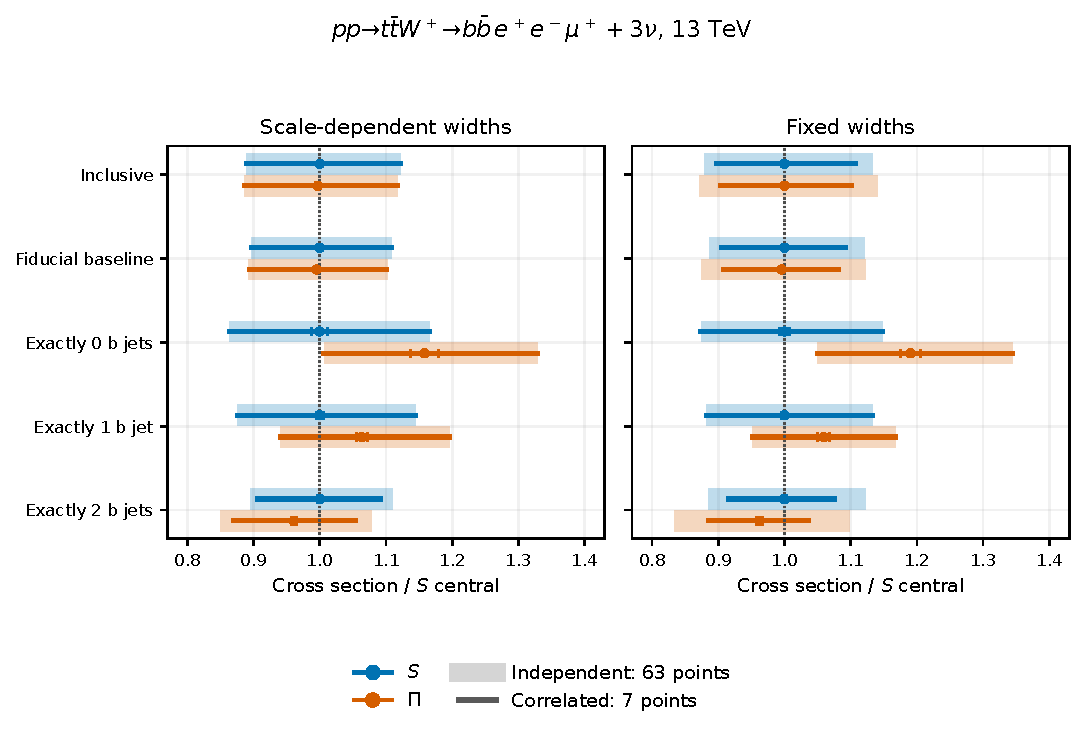
\includegraphics[width=\linewidth]{01_rates.pdf}
\caption{Inclusive and fiducial central predictions and scale envelopes.
Within each selection the numerical unit on the horizontal axis is the
$S$ central value for that width convention. Light thick ranges are I63,
thin solid ranges C7, and markers with small bars show the individual
central MC error. The normalization is a plotting reference, not an
estimated ratio error. The zero-/one-tag enhancement and two-tag decrease
are clearer than the inclusive difference.}
\label{fig:rates}
\end{figure}
\begin{figure}[htbp]\centering
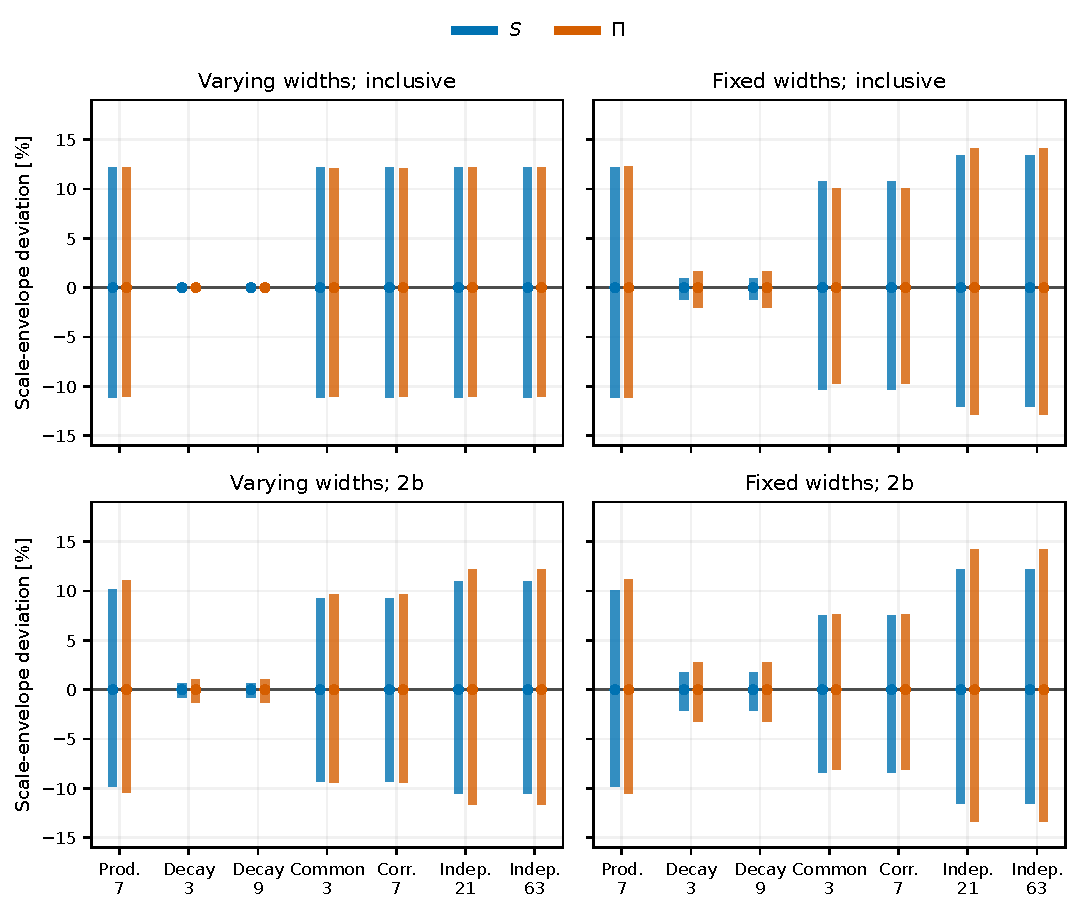
\includegraphics[width=\linewidth]{02_scale_prescriptions.pdf}
\caption{Scale-prescription comparison for inclusive and two-tag rates.
Each vertical range is the minimum/maximum relative to its own central
prediction; markers sit at zero. Fixed widths strengthen the decay-scale
response and its cancellation against production when scales are tied.
Independent variation recovers a larger envelope. The separate decay axes
do not further enlarge these particular integrated extrema.}
\label{fig:scales}
\end{figure}
\begin{figure}[htbp]\centering
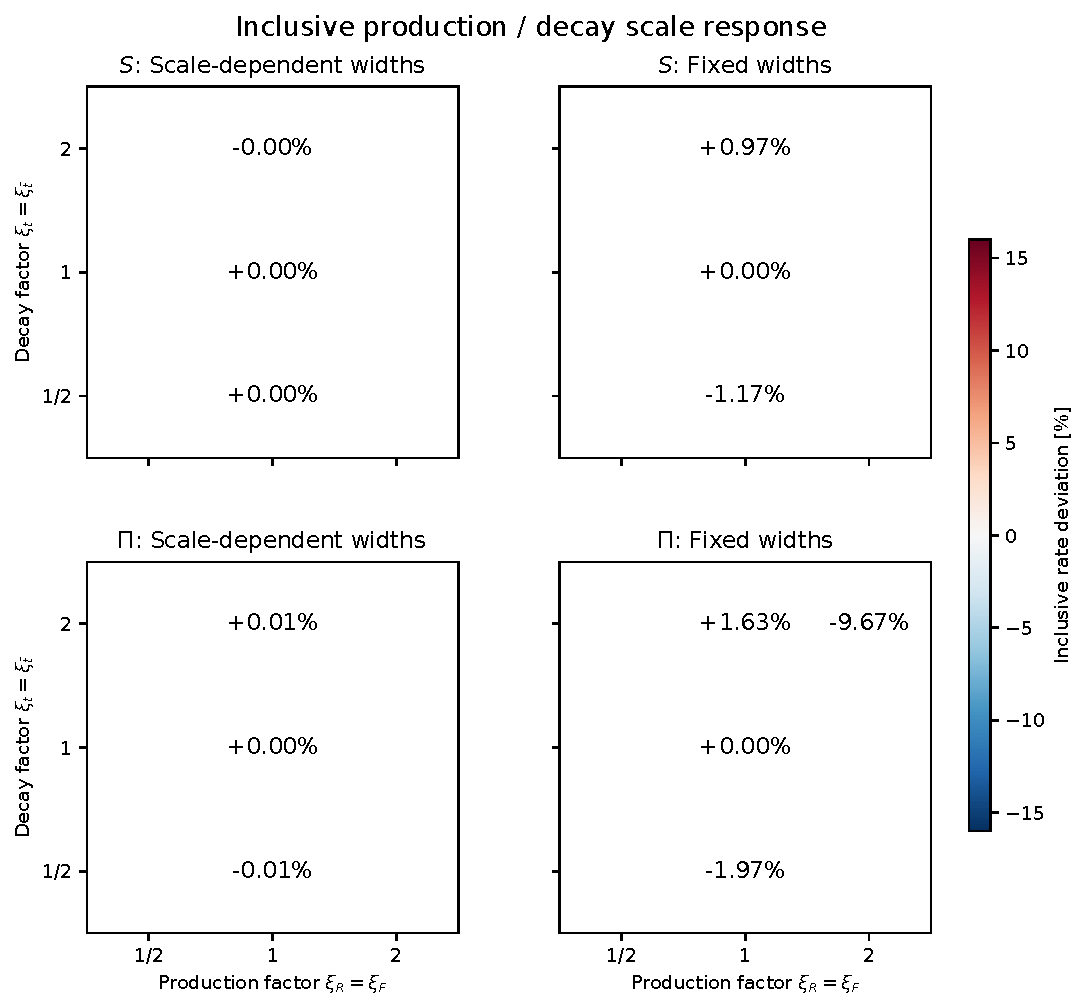
\includegraphics[width=.92\linewidth]{03_scale_response.pdf}
\caption{Inclusive scale-response slices, with production
$\xi_R=\xi_F$ and decay $\xi_t=\xi_{\bar t}$.
Each cell gives the percentage change relative to the corresponding
central run. Correlated Common3 follows the diagonal; independent
production/decay variations also reach off-diagonal cells. Near-flat decay
response with varying widths becomes a competing slope with fixed
widths. This is a response surface of the stored weights, not a
statistical covariance or a likelihood.}
\label{fig:response}
\end{figure}

\clearpage
\begin{figure}[htbp]\centering
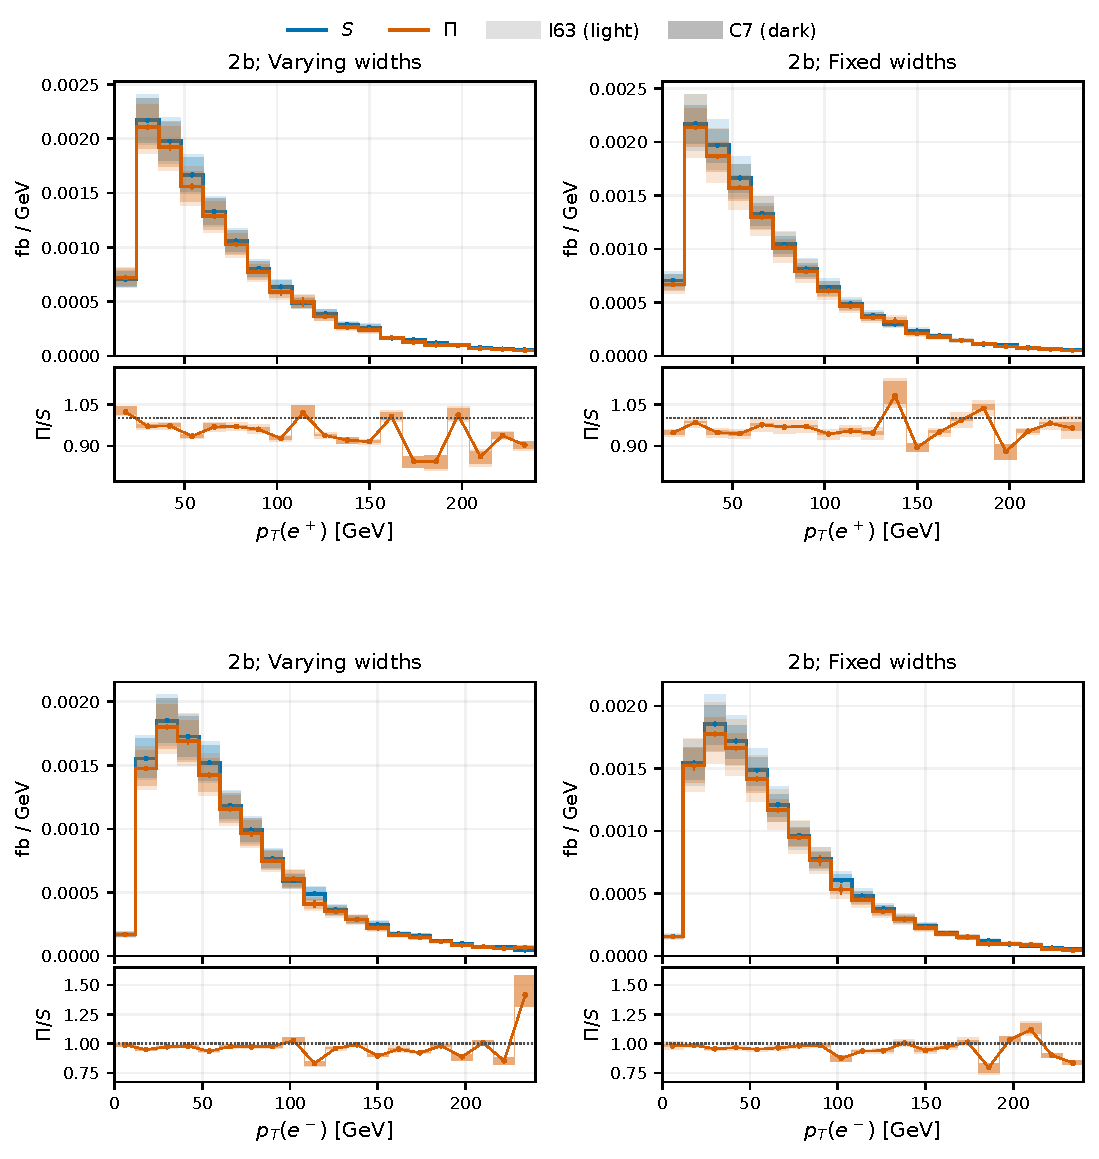
\includegraphics[width=\linewidth]{04_lepton_pt.pdf}
\caption{Two-tag electron and positron transverse-momentum spectra. Left:
scale-dependent widths; right: fixed widths. Upper panels show signed
absolute densities with per-run MC bars, light I63 and dark C7 bands.
Lower panels show the scale-matched $\Pi/S$ central ratio and envelopes;
no ratio MC errors are inferred. Tail fluctuations should be assessed
against the absolute-panel errors, not the ratio scale band alone.}
\label{fig:leptons}
\end{figure}
\begin{figure}[htbp]\centering
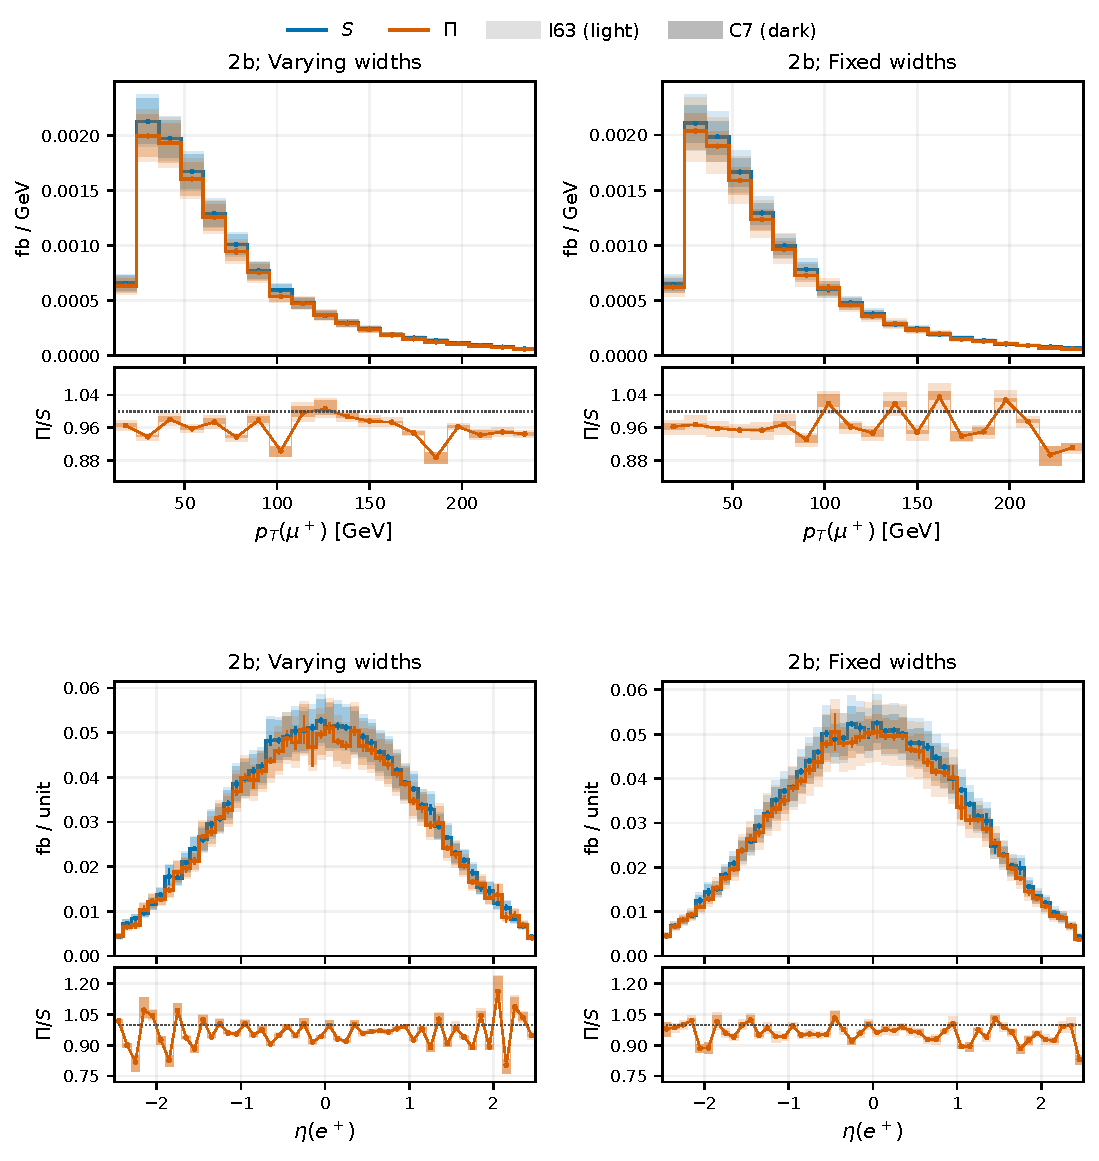
\includegraphics[width=\linewidth]{05_muon_eta.pdf}
\caption{Two-tag associated-muon transverse momentum and positron
pseudorapidity. Conventions are as in Fig.~\ref{fig:leptons}. The associated
lepton probes production and spin information, while the top-decay
positron also responds to decay selection. Identical central definitions
for the two width columns allow their variation-band changes to be
separated from their independently sampled central fluctuations.}
\label{fig:muon}
\end{figure}
\begin{figure}[htbp]\centering
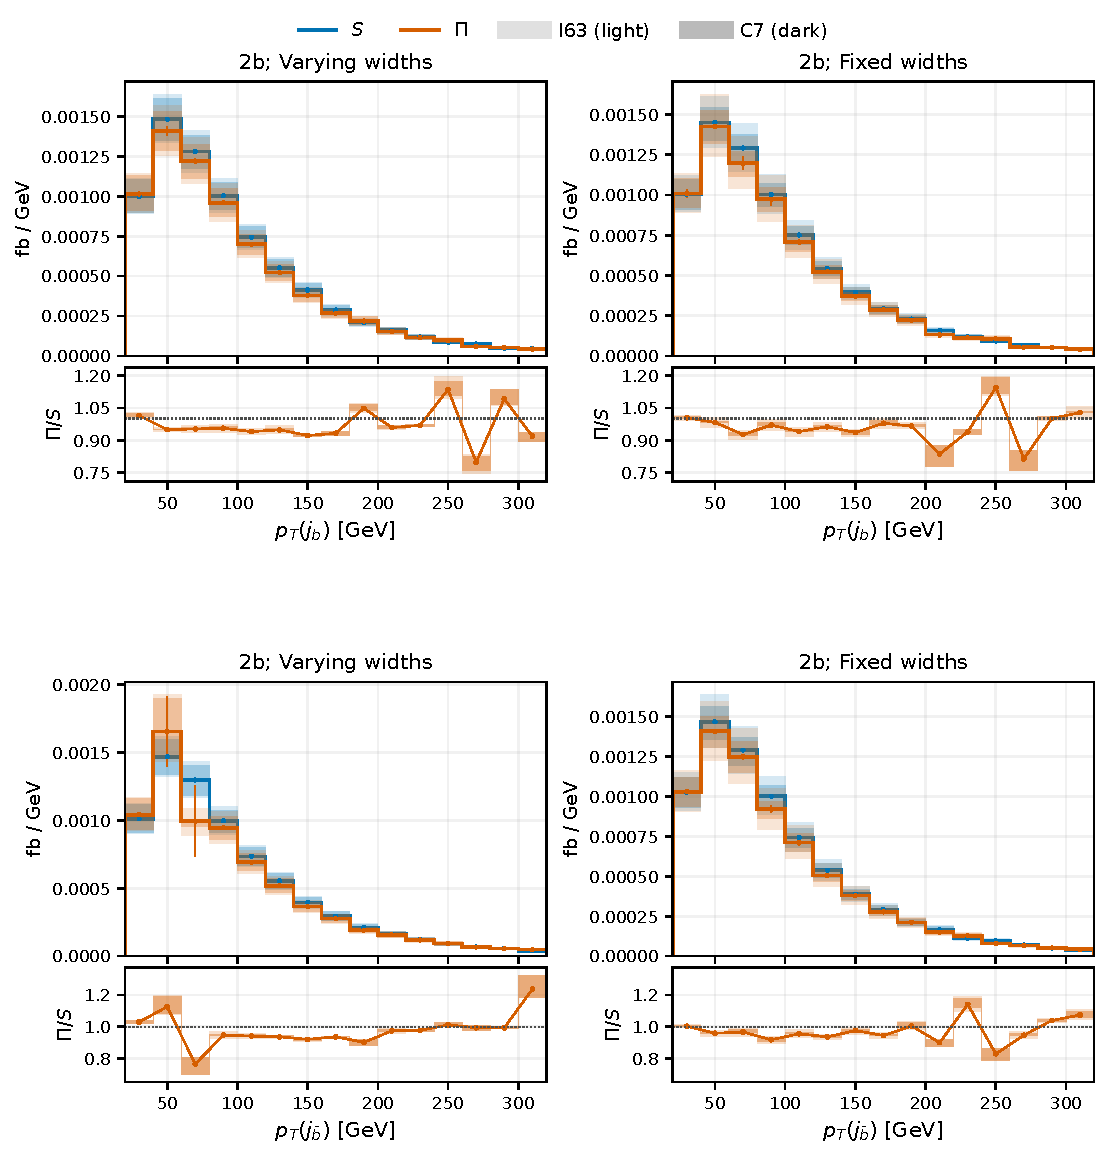
\includegraphics[width=\linewidth]{06_bottom_pt.pdf}
\caption{Separate accepted bottom- and antibottom-jet transverse momenta
in the two-tag category. Merged b--antibottom jets do not contribute.
The different acceptance thresholds for positive and negative top-decay
leptons can make the two selected jet spectra different even though the
jet acceptance cuts are identical. Bands and errors follow
Fig.~\ref{fig:leptons}; the upper spectra are not shape-normalized.}
\label{fig:bottom}
\end{figure}
\begin{figure}[htbp]\centering
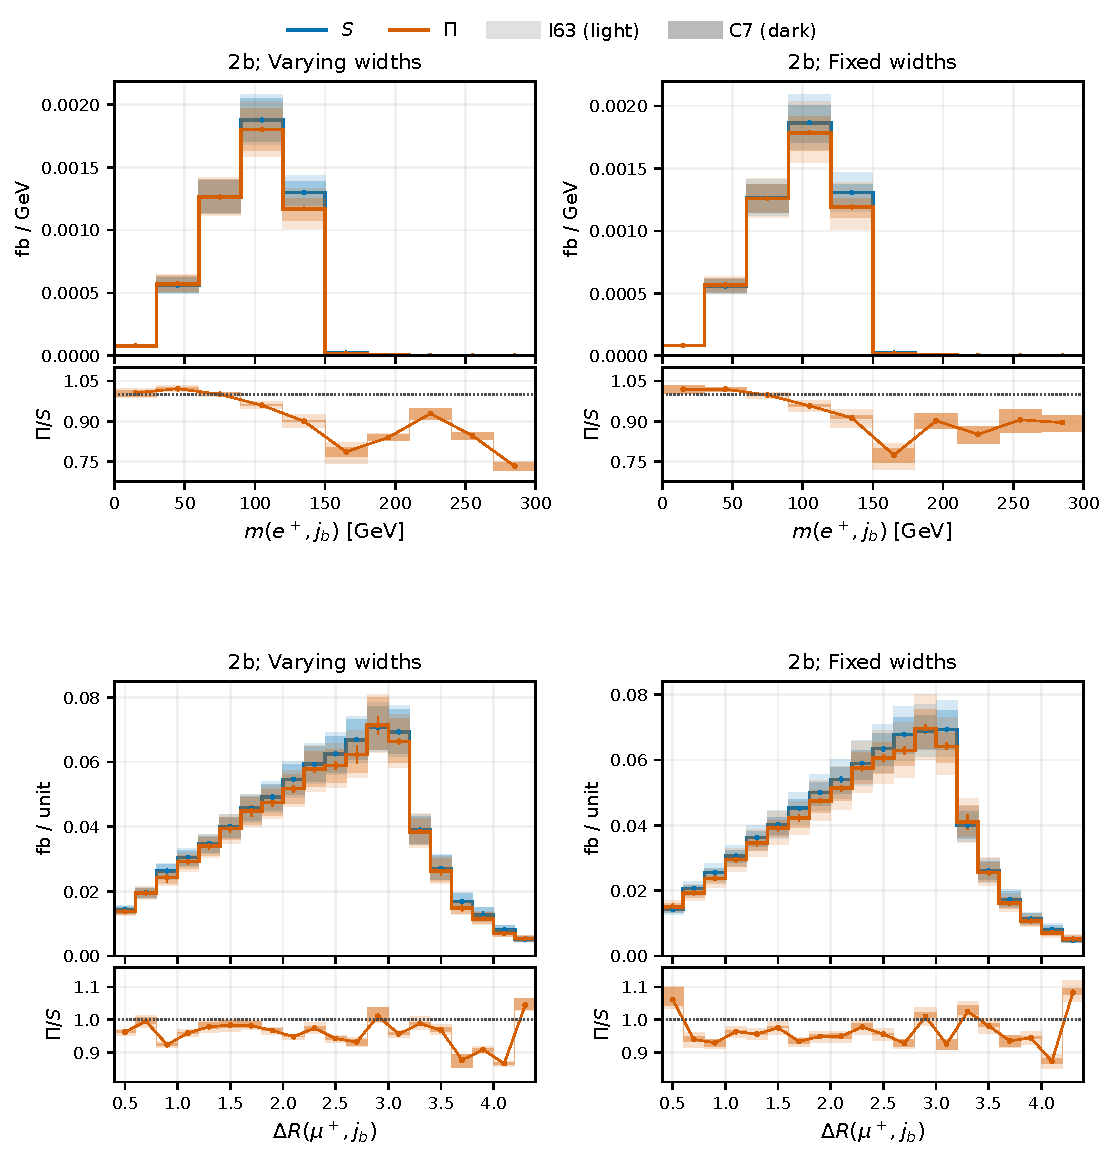
\includegraphics[width=\linewidth]{07_lepton_bottom.pdf}
\caption{Two-tag $m(e^+,j_b)$ and $\Delta R(\mu^+,j_b)$.
The invariant mass combines the top-decay positron and its bottom jet in
this specified flavour assignment; the jet can include recombined QCD
radiation. Bins beyond the approximately 152.6 GeV Born endpoint emphasize
radiative configurations. The angular plot provides a separate
production/decay correlation without a missing-momentum fit. Native bins
are retained; all displayed ratio envelopes use matched scale vectors.}
\label{fig:lepb}
\end{figure}
\begin{figure}[htbp]\centering
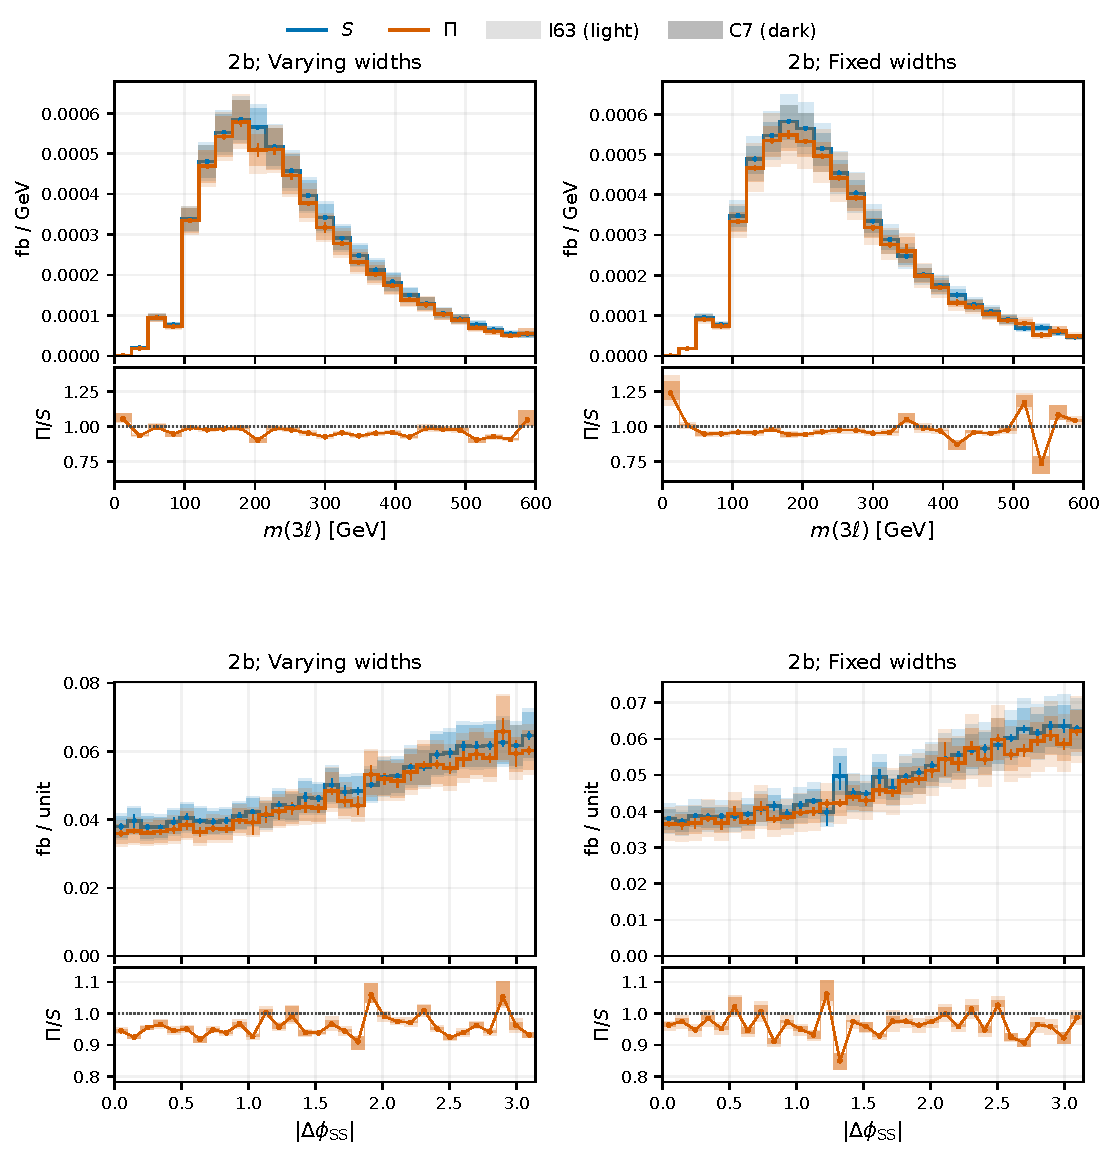
\includegraphics[width=\linewidth]{08_trilepton_angles.pdf}
\caption{Two-tag trilepton invariant mass and same-sign lepton azimuthal
separation, with the same absolute/ratio conventions. In this process the
same-sign pair is $e^+\mu^+$. These directly visible combinations provide
useful complementary checks to single-object spectra, without any
neutrino-root or parent-assignment minimization.}
\label{fig:trilepton}
\end{figure}
\begin{figure}[htbp]\centering
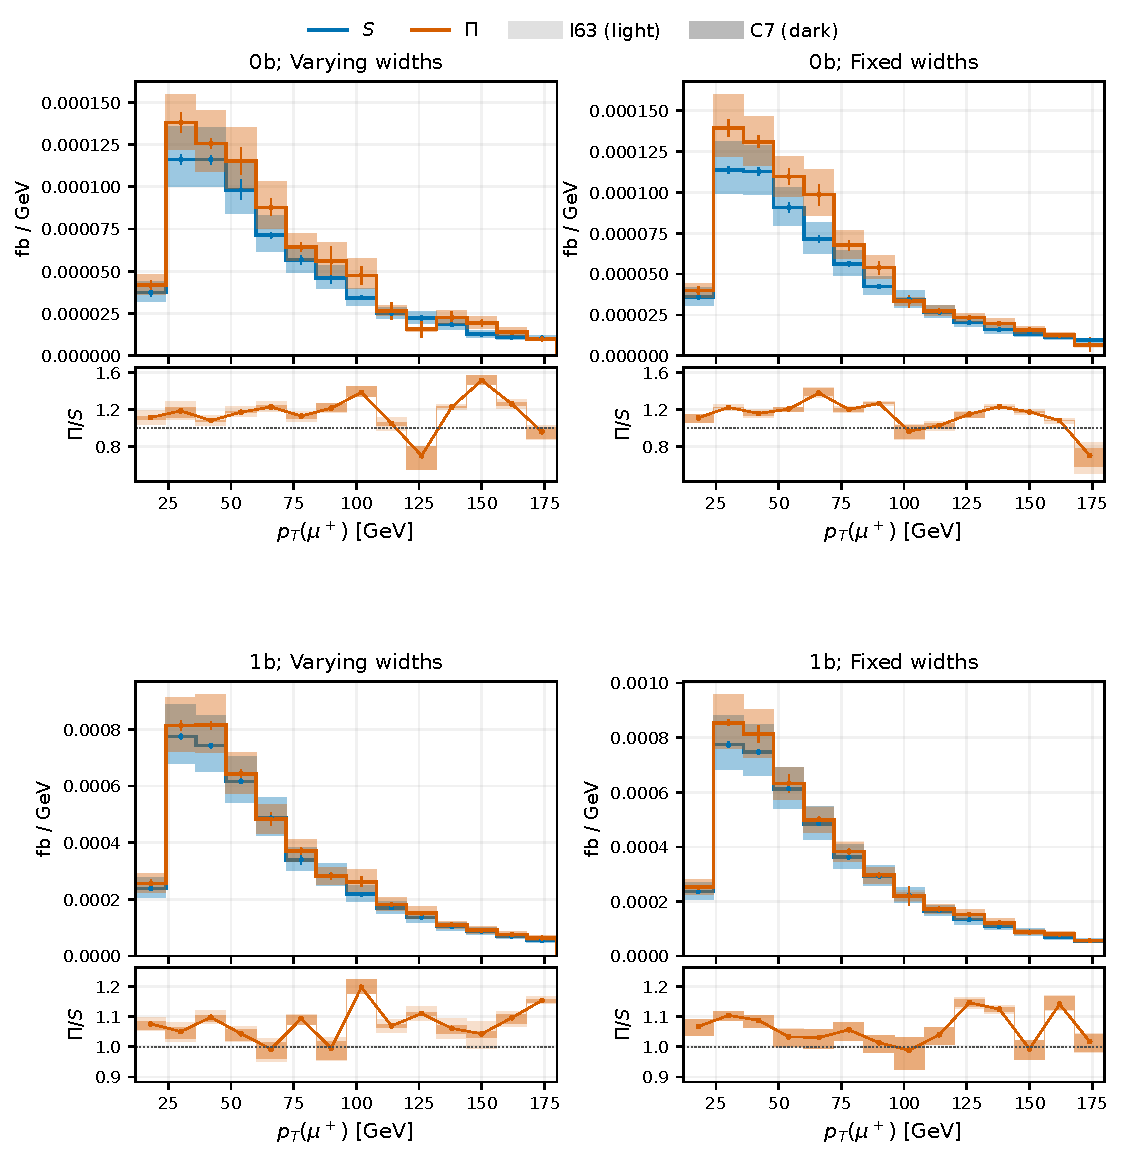
\includegraphics[width=\linewidth]{09_low_tag_categories.pdf}
\caption{Associated-muon transverse momentum in the exclusive zero-tag
and one-tag categories. Their integrated enhancements in $\Pi$ persist
in the collected rates, but the zero-tag differential sample is visibly
less precise. This figure displays that limitation rather than smoothing
or removing noisy native bins. Ratio shading is scale variation only;
MC uncertainty remains on the absolute spectra.}
\label{fig:lowtags}
\end{figure}

\clearpage
\appendix
\section{Reproducibility and interpretation limits}
The report directory contains the LaTeX source and generated PDF; nine
standalone PDF/PNG figures; archived input cards under \code{inputs/};
\code{results.json} with input SHA256 hashes, rate/ratio reductions and
explicit scale grids; \code{collected.npz} with all central values, MC
errors and scale weights; a figure manifest; and a full-catalogue
precision CSV. Input histograms were not edited or merged with estimates
of different observables. The collection verifies identical histogram
boundaries, unique complete scale labels, nominal/central-weight agreement,
the exclusive-tag closure at every scale point, and the archived fixed-width
settings. These are bookkeeping checks, not a convergence certification.

From the repository root, regenerate the reduction and figures with
\begin{verbatim}
python ttw_study/scripts/collect_decay_scale_report.py
python ttw_study/scripts/render_decay_scale_report.py
cd ttw_study/reports/decay_scales_20261019
pdflatex -interaction=nonstopmode -halt-on-error report.tex
pdflatex -interaction=nonstopmode -halt-on-error report.tex
\end{verbatim}
The prose interpretation is tied to the four collected runs and should be
reviewed if those inputs change. The render step uses native bins and
preserves the four scale coordinates in the order production $\mu_R$,
production $\mu_F$, top $\mu_R$, antitop $\mu_R$ even though the runtime
labels print \code{d-6} before \code{d6}.

The present sample does not include a direct-lepton-flavour sum, the
charge-conjugate $W^-$ process, PDF uncertainty, non-factorizable effects,
finite-width/off-shell effects, electroweak higher orders or a full NNLO
calculation. These omissions delimit what the quoted central agreements
and envelope comparisons mean; none can be supplied by expanding the
existing scale-point set. The old reconstruction instability was removed
at the analysis-definition level; the finite-statistics fluctuations still
visible here are not evidence by themselves for a new infrared-safety
failure.

\begin{thebibliography}{9}
\bibitem{MG5} J. Alwall et al.,
\emph{The automated computation of tree-level and next-to-leading order
differential cross sections, and their matching to parton shower simulations},
JHEP 07 (2014) 079, \href{https://arxiv.org/abs/1405.0301}{arXiv:1405.0301}.
\bibitem{MadFKS} R. Frederix, S. Frixione, F. Maltoni and T. Stelzer,
\emph{Automation of next-to-leading order computations in QCD: the FKS subtraction},
JHEP 10 (2009) 003, \href{https://arxiv.org/abs/0908.4272}{arXiv:0908.4272}.
\bibitem{ttW2020} G. Bevilacqua, H.-Y. Bi, H. B. Hartanto, M. Kraus and M. Worek,
\emph{The simplest of them all: $t\bar tW^\pm$ at NLO accuracy in QCD},
JHEP 08 (2020) 043, \href{https://arxiv.org/abs/2005.09427}{arXiv:2005.09427}.
\end{thebibliography}
\end{document}
